\chapter{Iteración 7}

\begin{abstract}
Esta iteración se orienta a consolidar sistemas ya introducidos y a extender la estructura
del recorrido con salas especiales. El trabajo se centra en refinar el sistema de enemigos y
el sistema de combate, además de cerrar la integración funcional de la sala de tienda, la
sala de tesoro y la sala secreta dentro de la generación procedural del mapa.
\end{abstract}

\section{Lista de funcionalidades}
La séptima iteración se plantea como una fase de consolidación sobre sistemas que en la
entrega anterior ya eran funcionales, pero todavía admitían una mejora clara en profundidad
jugable y en variedad de recorrido. El foco principal recae sobre combate y enemigos,
mientras que la incorporación de salas especiales amplía la estructura del mapa con espacios
de función diferenciada. Con el estado actual del proyecto, la iteración ya no se limita a
dejar estas salas encajadas a nivel estructural, sino que las conecta con contenido jugable
real y reglas de acceso específicas.

\begin{enumerate}
\item \textbf{Sistema de Enemigos.} Esta funcionalidad profundiza en el comportamiento
enemigo sobre la base ya creada anteriormente. Su alcance real consiste en diferenciar con
más claridad la respuesta táctica de cada arquetipo, introduciendo preparación visible del
ataque, desplazamientos de compromiso, recuperación tras empujes y una relación más fuerte
entre el contexto del arma del jugador y el daño final que recibe cada tipo de enemigo. A
esto se suma una mejor activación por sala y una integración más coherente con el sistema de
aparición ponderada por círculo y por tipo de habitación. En términos funcionales, la
feature hace que los enfrentamientos resulten más legibles y menos genéricos, ya que el
jugador puede anticipar mejor la intención del enemigo y adaptar su respuesta según el tipo
de amenaza al que se enfrenta.

\begin{figure}[H]
\begin{center}
\missingfigure{Sustituir por captura representativa del Sistema de Enemigos en la iteración 7}
% \includegraphics[width=.9\textwidth]{figures/iteracion7_sistema_enemigos.png}
\caption{Resultado visual de la feature Sistema de Enemigos en la iteración 7}
\label{fig:iteracion7-feature-enemigos}
\end{center}
\end{figure}

\item \textbf{Sistema de Combate.} Esta funcionalidad refina el combate del jugador para que
cada arma no solo tenga parámetros distintos, sino también una lectura más clara en su uso y
una interacción más rica con el resto de sistemas. El trabajo realizado en esta iteración
introduce ataques cargados para armas que lo requieren, proyectiles con comportamiento más
sofisticado y apoyo visual específico tanto en ataques cuerpo a cuerpo como en proyectiles.
Además, el sistema mantiene el contexto del arma y de la forma activa del jugador durante el
ataque, lo que facilita que otros componentes interpreten el impacto con mayor precisión. En
la práctica, esta ampliación hace que el combate se perciba como un sistema más expresivo,
con mejor retroalimentación y con una conexión más sólida entre entrada, ataque y efecto
producido en pantalla.

\begin{figure}[H]
\begin{center}
\missingfigure{Sustituir por captura representativa del Sistema de Combate en la iteración 7}
% \includegraphics[width=.9\textwidth]{figures/iteracion7_sistema_combate.png}
\caption{Resultado visual de la feature Sistema de Combate en la iteración 7}
\label{fig:iteracion7-feature-combate}
\end{center}
\end{figure}

\item \textbf{Sala de tienda.} Esta funcionalidad introduce una habitación especial dentro
de la generación del mapa con identidad propia y con señalización específica en el minimapa.
Su alcance real no se queda en la clasificación espacial de la habitación, sino que incorpora
contenido interactivo mediante puestos de compra, selección de objetos y precios asociados al
pool de drops del círculo actual. En términos funcionales, la tienda deja de ser una sala
marcada en el mapa y pasa a convertirse en un nodo de economía y preparación dentro de la
partida, conectado tanto con el inventario como con la progresión por objetos.

\begin{figure}[H]
\begin{center}
\missingfigure{Sustituir por captura representativa de la Sala de tienda en la iteración 7}
% \includegraphics[width=.9\textwidth]{figures/iteracion7_sala_tienda.png}
\caption{Resultado visual de la feature Sala de tienda en la iteración 7}
\label{fig:iteracion7-feature-tienda}
\end{center}
\end{figure}

\item \textbf{Sala secreta y de tesoro.} Esta funcionalidad amplía la distribución de salas
especiales con espacios que no siguen exactamente las mismas reglas de acceso que las salas
regulares. En la versión actual del proyecto, la sala de tesoro ya genera recompensas
recogibles, mientras que la sala secreta se resuelve como un espacio oculto accesible a
través de un muro rompible, reforzando la idea de descubrimiento. Esta línea de trabajo se
centra en hacer que el recorrido entre salas especiales deje de ser decorativo y pase a
tener recompensa e identidad propia dentro de la \textit{run}.

\begin{figure}[H]
\begin{center}
\missingfigure{Sustituir por captura representativa de la Sala secreta y de tesoro en la iteración 7}
% \includegraphics[width=.9\textwidth]{figures/iteracion7_salas_especiales.png}
\caption{Resultado visual de la feature Sala secreta y de tesoro en la iteración 7}
\label{fig:iteracion7-feature-salas-especiales}
\end{center}
\end{figure}
\end{enumerate}

La combinación de estas funcionalidades hace que la séptima iteración actúe como una capa de
consolidación y ampliación. Por un lado, refuerza la calidad táctica del combate y de los
enemigos; por otro, abre el mapa a recorridos más variados mediante salas especiales con un
papel diferenciado dentro de la partida y con impacto real sobre la economía, la exploración
y la progresión.

\section{Diseño}
El diseño de esta iteración parte de una necesidad doble: enriquecer la calidad de los
enfrentamientos y dar más valor estructural a determinadas salas dentro del recorrido
procedural. En ambos casos, la idea dominante fue evitar soluciones aisladas y reutilizar la
arquitectura ya existente para hacerla más expresiva sin perder coherencia con lo anterior.

\subsection{Diseño del sistema de enemigos}
La decisión principal fue reforzar la identidad táctica de cada tipo de enemigo mediante
patrones de ataque y movimiento más distinguibles. No bastaba con que hubiera variantes con
distinto daño o velocidad; era necesario que el jugador percibiera de forma clara cuándo un
enemigo iba a cargar, disparar o comprometer una embestida.

Por ello, el diseño de esta ampliación se orientó a introducir fases de preparación visibles,
desplazamientos de ataque más marcados y una respuesta al daño más sensible al arma empleada.
Con ello, el enemigo deja de ser únicamente una fuente de daño y pasa a actuar como una
pieza táctica reconocible dentro del encuentro.

\subsection{Diseño del sistema de combate}
El refinamiento del combate se diseñó bajo el criterio de mantener una lógica unificada para
todas las armas, pero permitiendo comportamientos suficientemente distintos como para que la
elección de una u otra tenga consecuencias jugables reales. A partir de ahí, se incorporó la
idea de ataques cargados y de proyectiles con capacidades adicionales, sin romper el modelo
de arma configurable que ya existía.

También se dio importancia al \textit{feedback} visual del ataque. Si el sistema pretendía
ser más expresivo, la respuesta en pantalla debía acompañar ese aumento de complejidad. Por
eso, el diseño no se limita a parámetros de daño o alcance, sino que contempla también
trazos, partículas y apoyos visuales ligados a la ejecución del ataque.

\subsection{Diseño de la sala de tienda}
La sala de tienda se diseñó como una categoría espacial propia dentro del conjunto de salas
terminales del mapa. La decisión importante aquí fue integrarla en la misma fase de
selección procedural que otras salas especiales, en lugar de tratarla como una excepción
colocada manualmente después.

Este enfoque hace que la tienda forme parte natural del reparto del recorrido y permite que
su identidad visual y estructural quede resuelta desde el propio generador de mapa. Sobre esa
base, la sala puede alojar contenido de compra sin depender de montaje manual en cada
variación visual de habitación.

\subsection{Diseño de la sala secreta y de tesoro}
La lógica de estas salas se diseñó para reforzar la exploración y la recompensa. La sala de
tesoro se concibe como un nodo especial identificado dentro del mapa, mientras que la sala
secreta requiere además un tratamiento distinto en su accesibilidad para que su descubrimiento
no se perciba igual que el de una habitación regular.

Por ello, el diseño introduce tipos de sala específicos y reglas de conexión diferenciadas,
de forma que la presencia de estas habitaciones no solo cambie el icono mostrado en el mapa,
sino también la lectura espacial del recorrido.

\section{Implementación}
La implementación de esta iteración se repartió entre el refinamiento de sistemas de acción
y la ampliación del generador procedural con nuevos tipos de sala. Aunque a nivel funcional
las features parecen distintas, todas comparten un mismo objetivo: hacer que el juego
responda con más riqueza al contexto en el que se produce cada evento.

\subsection{Implementación del sistema de enemigos}
La ampliación del comportamiento enemigo se apoyó sobre todo en \texttt{EnemyController},
\texttt{EnemyProjectile}, \texttt{EnemyHealth} y \texttt{CircleDefinition}. En
\texttt{EnemyController} se refuerzan los patrones diferenciados de enemigos normales,
voladores y tanque mediante tiempos de preparación, ataques con embestida, disparos a
distancia, recuperación de \textit{knockback} y señales visuales previas al ataque.

Además, el sistema se integra de forma más estrecha con el contexto del arma del jugador.
Para ello se consulta \texttt{DamageSourceContext}, lo que permite ajustar multiplicadores de
daño en función del arma concreta y de la forma activa. A esto se suma una mejor relación
con la activación por sala, el estado dormido inicial y la selección ponderada de enemigos
desde la definición del círculo y del tipo de habitación.

\subsection{Implementación del sistema de combate}
El refinamiento del combate se apoya en \texttt{PlayerCombatController},
\texttt{WeaponDefinition}, \texttt{Projectile}, \texttt{MeleeHitbox},
\texttt{PlayerChargeAttackVisual} y los componentes visuales asociados a proyectiles y
golpes de melé. \texttt{PlayerCombatController} mantiene la selección de arma según la forma
del jugador y amplía el flujo de ataque para soportar ataques cargados, donde el daño final
depende del tiempo de preparación acumulado.

En paralelo, la implementación añade apoyo visual para hacer más legible cada acción:
trazos de ataque en melé, indicadores de carga y estelas o partículas ligadas al
desplazamiento de proyectiles. El sistema conserva además el contexto completo del ataque
mediante \texttt{DamageSourceContext}, lo que permite conectar el golpe con otros sistemas
que interpretan el impacto más allá del valor numérico del daño.

\subsection{Implementación de la sala de tienda}
La base técnica de la sala de tienda se apoya en \texttt{MapGenerator}, \texttt{Cell} y en
la configuración de puertas y muros de \texttt{Room}. \texttt{MapGenerator} selecciona un
índice específico para esta sala dentro del conjunto de habitaciones terminales, le asigna
un tipo propio y actualiza su representación visual en el mapa mediante iconografía
dedicada.

Después, esa información se propaga al resto del sistema a través del tipo de sala
almacenado en la celda, lo que permite que puertas, muros y minimapa la interpreten como una
categoría distinta. Sobre esa base, \texttt{Room} busca o instancia un \texttt{ShopManager}
al cargar la variación visual de la habitación, y este a su vez genera \texttt{ShopStand}
con objetos y precios derivados del círculo actual. Con ello, la tienda queda integrada como
espacio funcional y no solo como tipo de sala.

\subsection{Implementación de la sala secreta y de tesoro}
La incorporación de salas especiales se apoya también en \texttt{MapGenerator}, que reserva
índices específicos para estas habitaciones y actualiza su \texttt{RoomType} dentro de cada
\texttt{Cell}. En el caso de la sala secreta, la selección se realiza con una lógica propia
que busca posiciones no ocupadas y con suficiente proximidad estructural al resto del mapa
para poder insertarla como espacio oculto.

Por otra parte, \texttt{Room} utiliza el tipo de sala para condicionar la colocación de
puertas. Esto permite que la sala secreta no siga exactamente el mismo patrón de acceso que
una sala regular, reforzando su papel como espacio de descubrimiento. Cuando se detecta una
conexión hacia una sala secreta, se coloca un \texttt{BreakableWall} que, al destruirse,
crea la puerta definitiva y mantiene la coherencia con el sistema de cierre y apertura de la
habitación.

En paralelo, la sala de tesoro se conecta con \texttt{TreasureManager} y
\texttt{TreasureStand} para poblar recompensas al instanciar la sala.

\section{Seguimiento y control}
El seguimiento de esta iteración estuvo muy condicionado por la naturaleza de las features
planificadas. Dos de ellas, sistema de combate y sistema de enemigos, provenían de una
replanificación deliberada tras comprobar en la iteración 5 que su complejidad real era mayor
de la estimada al principio. En consecuencia, el control en esta fase no consistió en abrir
trabajo completamente nuevo, sino en cerrar con más profundidad aspectos que ya se habían
validado como base funcional.

La iteración permitió completar ese refinamiento sin perder de vista el alcance temporal
disponible. Al mismo tiempo, la incorporación de sala de tienda y de salas especiales añadió
contenido nuevo, pero en un ámbito más acotado y sobre una arquitectura ya preparada para ello.
Desde el punto de vista de planificación, esta combinación permitió equilibrar consolidación y
ampliación, y confirmó que la división previa de features fue necesaria para ajustar mejor el
trabajo al esfuerzo real que exigían.

\section{Resultados}
El resultado de la iteración fue el cierre de una capa jugable más rica tanto en combate como
en estructura de recorrido. Por un lado, combate y enemigos ganaron profundidad, legibilidad
y capacidad de respuesta al contexto. Por otro, las salas especiales dejaron de ser meras
variantes espaciales y pasaron a aportar economía, recompensa, exploración oculta y
exploración oculta.

De forma resumida, al final de esta iteración se había conseguido:

\begin{itemize}
    \item reforzar la diferenciación táctica entre enemigos normales, voladores y tanque;
    \item ampliar el combate con ataques cargados y apoyos visuales más expresivos;
    \item mantener el contexto del arma y de la forma del jugador a lo largo del impacto;
    \item integrar la sala de tienda como espacio funcional de compra ligado al inventario y al círculo actual;
    \item incorporar sala de tesoro y sala secreta con reglas de acceso y recompensa diferenciadas.
\end{itemize}

Desde el punto de vista del desarrollo global, esta iteración resulta importante porque
mejora la calidad del enfrentamiento y empieza a enriquecer el recorrido más allá de la
simple sucesión de salas regulares. A partir de aquí, el proyecto dispone ya de una estructura
de partida más completa, en la que el avance por el mapa no solo cambia la disposición de las
habitaciones, sino también la clase de interacción y de recompensa que cada una puede ofrecer.

\begin{figure}[htbp]
\begin{center}
% \missingfigure{Sustituir por el diagrama UML de resultado de la iteración 7}
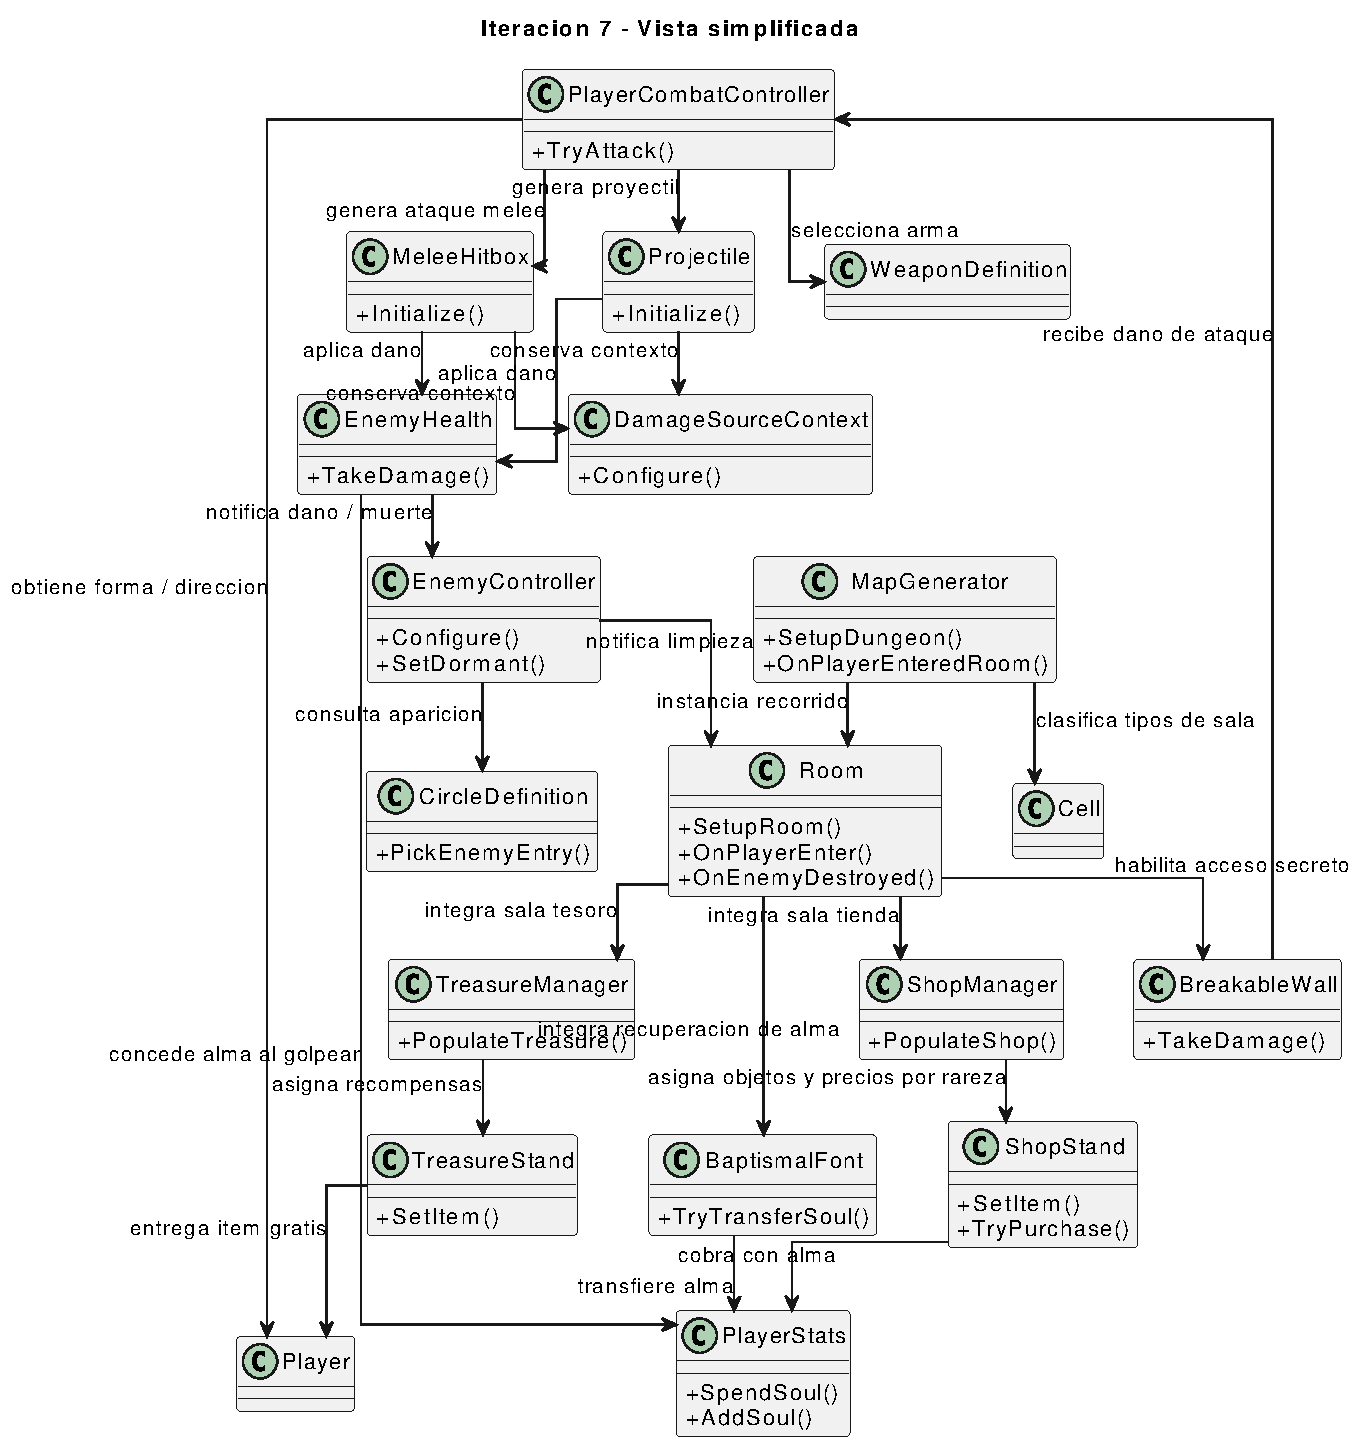
\includegraphics[width=\textwidth]{figures/iteracion7_resultado_uml.pdf}
\caption{Diagrama UML de resultado de la iteración 7}
\label{fig:uml-resultado-iteracion7}
\end{center}
\end{figure}
